\begin{figure}[H]
    \centering
    \begin{adjustbox}{width=10.5cm,center}
      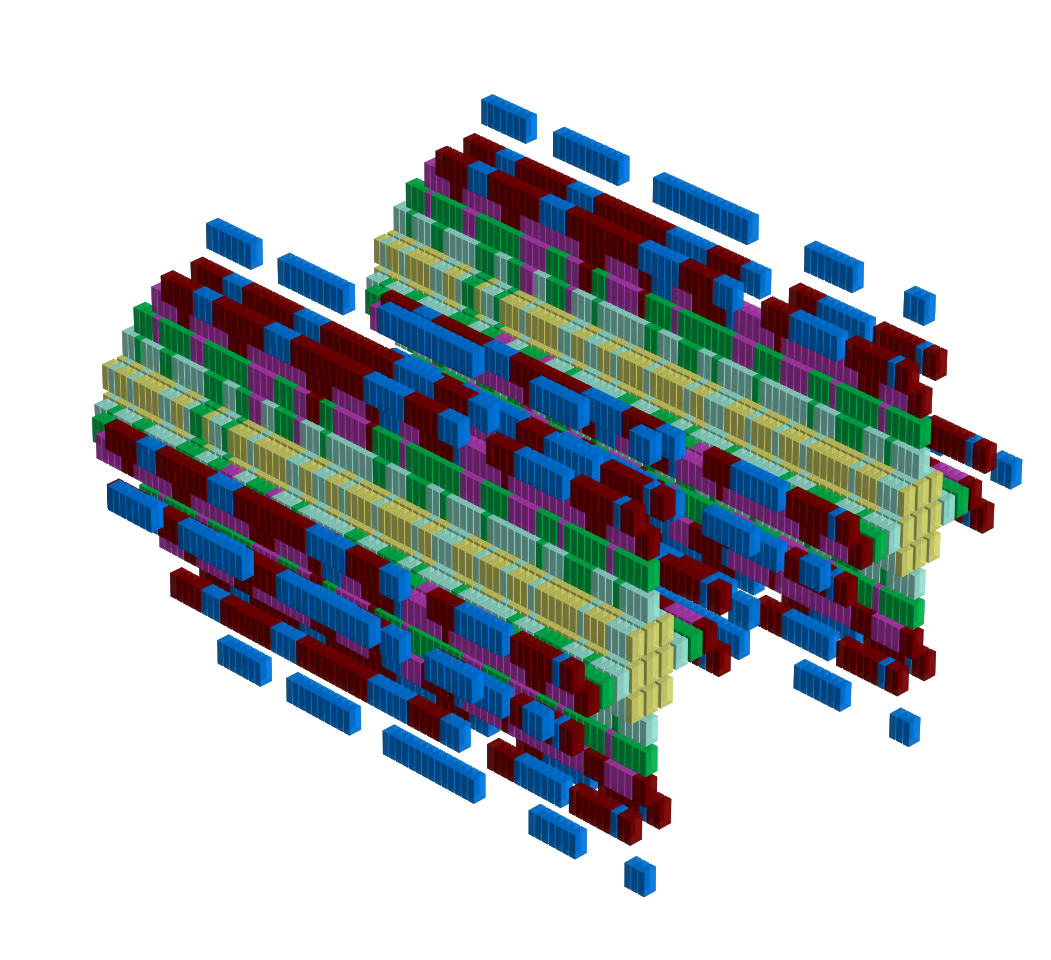
\includegraphics[width=10cm]{src/pulsespeed/pattern0-45.png}%
    \end{adjustbox}
    \begin{adjustbox}{width=10.5cm,margin=0cm -2cm}
      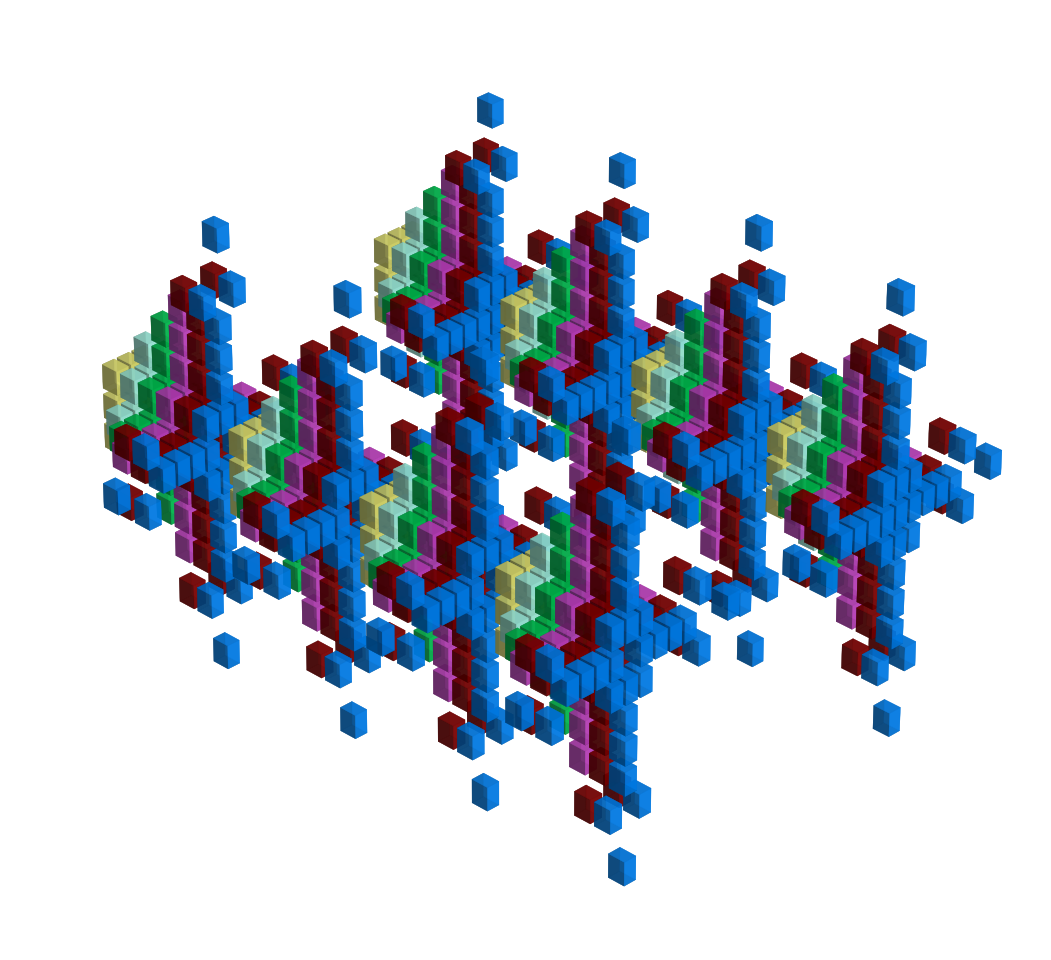
\includegraphics[width=10cm]{src/pulsespeed/pattern1-45.png}%
    \end{adjustbox}
    \caption{Effect of low and high values for Pulse Speed}
\end{figure}
\clearpage
\section*{pulse speed} 
\label{sec:pulse_speed}
\lstset{style=6502Style}
\lstset{ 
   aboveskip=5pt,
   belowskip=0pt,
}

\begin{definition}[Jeffrey Says]
\setlength{\intextsep}{0pt}%
\setlength{\columnsep}{3pt}%
\begin{wrapfigure}{l}{0.12\textwidth}

\includegraphics[width=\linewidth]{src/callout/psych.png} 
\end{wrapfigure}
\small
\textbf{P to activate:} Usually if you hold down the button
you get a continuous stream. Setting the Pulse Speed allows you to
generate a pulsed stream, as if you were rapidly pressing and
releasing the FIRE button.
\\
\end{definition}




\clearpage
\textbf{Lines 1189-1231. \icode{\textbf{MaybePPressed}}} 
\begin{lstlisting}[caption=From \icode{CheckKeyboardInput}.]
MaybePPressed   
  CMP #KEY_P ; P pressed
  BNE MaybeHPressed

  ; P pressed.
  LDA #PULSE_SPEED
  STA currentVariableMode
  RTS 
\end{lstlisting}
\textbf{Lines 1189-1231. \icode{\textbf{UpdateVariableDisplay}}} 
\begin{lstlisting}[caption=From \icode{CheckKeyboardInputForActiveVariable}. Pressing the \icode{<} and > keys increments and
decrements the value in presetValueArray pointed to by \icode{X}\, i.e. \icode{currentVariableMode}.]
UpdateVariableDisplay   
  LDA #>SCREEN_RAM + $03D0
  STA colorBarColorRamHiPtr
  LDA #<SCREEN_RAM + $03D0
  STA colorBarColorRamLoPtr
  LDX currentVariableMode
  LDA lastKeyPressed
  CMP #$2C ; > pressed?
  BNE MaybeLeftArrowPressed
  ; > pressed, increase the value bar and write
  ; it to the approiate place in presetValueArray
  INC presetValueArray,X
  LDA presetValueArray,X
  ; Make sure we don't exceed the max value.
  CMP maxValueForPresetValueArray,X
  BNE MaybeInColorMode
  DEC presetValueArray,X
  JMP MaybeInColorMode
\end{lstlisting}
\textbf{Lines 1189-1231. \icode{\textbf{presetValueArray}}} 
\begin{lstlisting}[basicstyle=\ttfamily\scriptsize,caption=From \icode{ActivateSequencer}.]
presetValueArray
unusedPresetByte        .BYTE $00
smoothingDelay          .BYTE $0C
cursorSpeed             .BYTE $02
bufferLength            .BYTE $1F
pulseSpeed              .BYTE $01; <-- Pulse Speed is here at position $04.
indexForColorBarDisplay .BYTE $01
lineWidth               .BYTE $07
sequencerSpeed          .BYTE $04 
pulseWidth              .BYTE $01
baseLevel               .BYTE $07
presetColorValuesArray  .BYTE BLACK,BLUE,RED,PURPLE,GREEN,CYAN,YELLOW,WHITE
trackingActivated       .BYTE $FF
lineModeActivated       .BYTE $00
presetIndex            .BYTE $05
\end{lstlisting}
\clearpage

\textbf{Lines 1189-1231. \icode{\textbf{presetValueArray}}:} 
 This is where the presets get loaded to. It represents the data structure
 for the presets.currentVariableMode is an index into this data structure
 when the user adjusts settings.
\clearpage


\clearpage
\begin{lstlisting}[caption=From \icode{MainInterruptHandler}.]
DecrementPulseSpeedCounter   
        DEC currentPulseSpeedCounter
        BEQ RefreshPulseSpeed
        JMP DrawCursorAndReturnFromInterrupt
        ; Returns

RefreshPulseSpeed   
        LDA pulseSpeed
        STA currentPulseSpeedCounter
        LDA pulseWidth
        STA currentPulseWidth

        ; Finally, update the pixel buffers with a byte
        ; each for the current pattern.        
UpdatePixelBuffersForPattern    
        INC currentStepCount
        LDA currentStepCount
        CMP bufferLength
        BNE UpdateBaseLevelArray

        LDA #$00
        STA currentStepCount
\end{lstlisting}
\clearpage

\textbf{Lines 1189-1231. \icode{\textbf{DisplayPresetMessage}}:} 
 This is where the presets get loaded to. It represents the data structure
 for the presets.currentVariableMode is an index into this data structure
 when the user adjusts settings.
\clearpage

